\section{Results}

In this chapter different results are shown.

\subsection{Lookup table}
In Figure \ref{fig:LUTsliceC2C} a visualization of a slice with a $D_{wake}$ of 230m and a $U_{fs}$ of 8m/s is shown. When looking at the $y_{C2C}$ it can be seen that DELs are significantly higher with partial wake overlap, but with larger negative $\gamma$ this effect is less extreme. Slices for other $D_{wake}$ and $U_{fs}$ show similar behavior. In Figure \ref{fig:LUTsliceDw} a slice with a $y_{C2C}$ = 0m and a $U_{fs}$ of 8m/s is shown. Here it is interesting to see that the effect of yaw is not symmetrical around $\gamma$ = 0deg. It is also noticeable that the lowest DEL value is around 10 to 20 degrees.  

\begin{figure}
	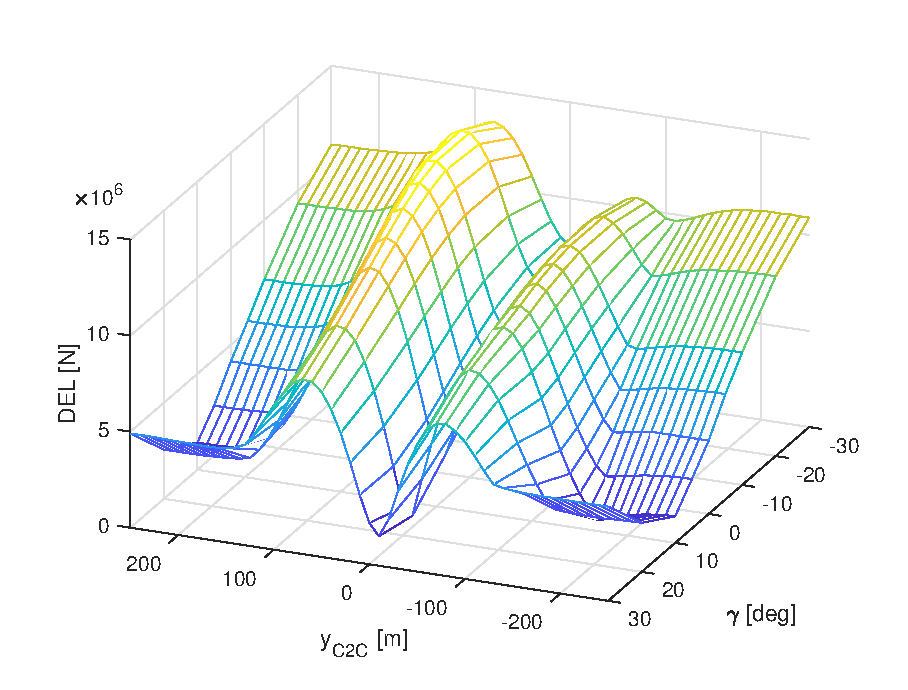
\includegraphics[width=\linewidth]{./Figures/LUTslice_Dw230_Ufs8.eps}
	\caption{Slice of the lookup table with a $D_{w}$ of 230m and a $U_{fs}$ of 8m/s }
	\label{fig:LUTsliceC2C}
\end{figure}

\begin{figure}
	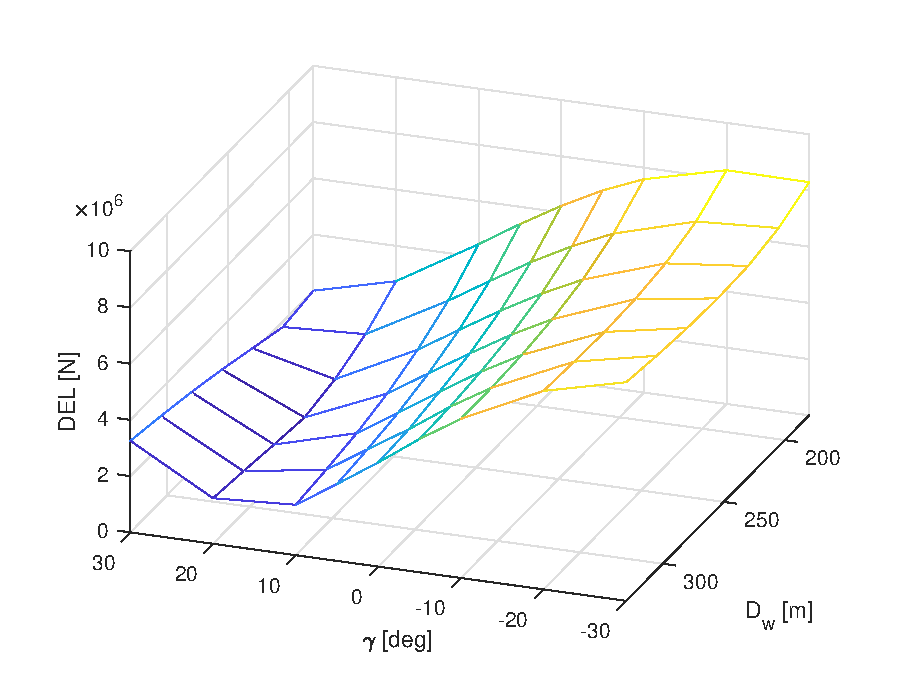
\includegraphics[width=\linewidth]{./Figures/LUTslice_yWake0_Ufs8.eps}
	\caption{Slice of the lookup table with a $y_{C2C}$ of 0m and a $U_{fs}$ of 8m/s }
	\label{fig:LUTsliceDw}
\end{figure}

\subsection{Simulation cases}
\label{sec:Simulation cases}
The two reference cases as described in section \ref{sec:Case studies} are shown in Table \ref{tab:Case results}. The cases with downgraded power are also shown in this table. The case with PREF on 90\% is shown as an example of the full optimization process. Figure \ref{fig:config90pct} shows the final turbine configuration for this optimization. 

\begin{table*}[p]
	\caption{Power and DEL values for greedy control and power-only optimization}
	\centering
	\label{tab:Case results}
	\begin{tabular}{rrc}
		\hline
		& Power [MW] & DELs \\ 
		\hline
		Greedy control & 12.42 & 13.22 \\
		Maximum power & 5.94E7 & - \\
		\hline
		\% of 13.22 & Percentage Pref & Percentage DEL\\
		\hline
		100 & -9.8E-4 & +5.72 \\
		90 & -8.4E-5 & -25.44 \\ %11.9
		80 & -1E-6 & -27.01 \\ %10.576
		70 & +3.2E-5 & -28.06 \\ %9.2
		60 & -2.6E-4 & -24.26 \\ %7.932
		50 & -1E-4 & -29.72 \\ %6.61
	\end{tabular}
\end{table*}

\begin{figure*}[p]
	\centering
	\includegraphics[trim=0cm 4cm 0cm 4cm, clip=true, width=0.9\linewidth]{./Figures/{Configuration_Pref11.9}.eps}
	%\vspace{-75pt}
	\caption{Turbine configuration after optimization with $P_{ref}$ at 90\%. }
	\label{fig:config90pct}
\end{figure*}

\begin{figure*}[p]
	\centering
	\includegraphics[width=0.85\linewidth]{./Figures/{Optimization_Pref11.9}.eps}
	\caption{Loads and power during optimization with $P_{ref}$ at 90\%. }
	\label{fig:optimization90pct}
\end{figure*}
